% schwartz-christoffel stuff

\section{Introduction}

Here we formulate a conformal mapping from the domain of the problem (the $W$ domain) to a domain on which it is easier to smooth (which we denote $W^*$.) We elaborate on what was alluded to in \cite{eilerstalk}: using the \sch mapping to transform our domain to another in order to perform smoothing. 

Given some complicated region that it is difficult to smooth over, one approach is to transform the domain in which the problem resides. So, for example, one could transform a region into a rectangle, circle or other familiar shape to avoid the problems such as leakage. In this spirit, we wish to find some mapping such as $\phi$ in \fig{simpledia}.

This kind of approach is appealing since it allows one to use existing techniques in the transformed domain (\emph{ie.} not having to resort to reformulating models in the manner of \cite{wangranalli}.) It also feels more natural to treat the domain as if it were made of silly putty and simply squash the region into the shape required to perform analysis.

% Simple diagram showing the mapping
\begin{figure} [htbp]
\centering
\includegraphics[scale=0.3]{sc/figs/simpledia.pdf}
\caption{An example of a transformation; the function $\phi$ takes the points in the rectangle and maps them to the region on the left.}
\label{simpledia}
\end{figure}

The \sch mapping offers such a transformation; it takes some arbitrary polygon and maps it to some specified shape. Commonly this is the upper half-plane ($H^+$), a rectangle or the unit disk. This is achieved in the $H^+$ case by taking the vertices of the polygon and mapping them to points on the real line (see \fig{reallinedia}.) This can be thought of as ``unwrapping'' the polygon onto the real line. For the unit disk case, we take points on the circle bounding the unit disk and map vertices on the polygon to those points (see \fig{unitdiskdia}.) One can think of this as adding control points to the unit circle and then altering the angles. The rectangular case is somewhat similar to the unit disk in that extra points are added to the boundary and the angles of these points tightened until the shape is identical to the polygon.

% Diagram showing upper half plane to polygon
\begin{figure} [tbp]
\centering
\includegraphics[scale=0.6]{sc/figs/reallinedia.pdf}
\caption{A mapping of the upper half-plane to the polygon. The vertices ($w_k$) are the result of applying $\phi$ to the points on the real line ($w^*_k$). The boundary of the polygon is mapped to the real line. Note that the final vertex, $w^*_6$ is mapped to the point $\infty$ on the real line.}
\label{reallinedia}
\end{figure}

% Diagram showing unit disk to polygon
\begin{figure} [tbp]
\centering
\includegraphics[scale=0.6]{sc/figs/unitdiskdia.pdf}
\caption{A mapping of the upper half-plane to the polygon. The vertices ($w_k$) are the result of applying $\phi$ to the points on the real line ($w^*_k$). The boundary of the polygon is mapped to the boundary of the unit disk.}
\label{unitdiskdia}
\end{figure}

The goal is to transform the domain with the complex boundary, then perform smoothing in the transformed domain. The procedure we wish to perform is as follows:

\begin{enumerate}
\item Determine the domain over which we would like to smooth, $W$. This could be the region or a bounding box around it.

\item Compute the \sch transform of $W$ to get $W^*$. To obtain the function, $\phi$.

\item Map the co-ordinates of the datapoints in $W$ to $W^*$.

\item Fit the GAM to the data in $W^*$.

\item Perform any further inference (in $W$ or $W^*$, since there is a 1-1 mapping between them.)
\end{enumerate}

The second section of this chapter explains the technical details of the mapping. The third section gives results of some simulations and the final section summarises the results and draws conclusions from them.

\section{Technical details}

This section gives some of the mathematical and computational details required to calculate the \sch mapping. The primary reference is the extremely thorough work of \cite{driscoll}, which covers almost all aspects of the \sch transform.

\subsection{Nomenclature}

We first define a polygon formally and its associated quantities as they will be referred to throughout the rest of the chapter.

A polygon, $\Gamma$, is a collection of vertices $w_1, w_2,\dots,w_n$ and interior angles $\alpha_1\pi, \alpha_2\pi, \dots, \alpha_n\pi$. For convenience we define $w_{n+1} = w_1$ and $w_0=w_n$. Numbering of vertices is anti-clockwise. The angles are such that $\alpha_k \in (0,2]$ and we require:
\begin{equation}
\sum_{k=1}^n (1-\alpha_k) = 2.
\end{equation}
We also define the exterior angle, $\theta_k\pi$, as given by $(1-\alpha_k)\pi$ (see \fig{anglediagram}.) It is the exterior angle that is of interest to us here.

% Diagram showing the exterior/interior angle relationship.
\begin{figure} [bp]
\centering
\includegraphics[scale=0.6]{sc/figs/anglediagram.pdf}
\caption{The external angle $\theta_k$ is associated with the vertex $w_k$. The internal angle is given by $\alpha_k$. Shading indicates the inside of the polygon.}
\label{anglediagram}
\end{figure}

The boundary of the polygon is denoted by $\Gamma$. We refer to two domains the $W$ and the $W^*$, denoting the original domain ($\Gamma$) and the transformed domain (of the plane, unit disk or rectangle) respectively. 

Vertices on the polygon are denoted as $w_k$ and those in the transformed domain are denoted as $w^*_k$ (the \emph{prevertices}.) In general a point in the polygon's original domain is denoted as $w$ and in the transformed domain as $w^*$.

We use the function $\phi$ to map from the transformed domain to the polygon (\emph{ie.} $\phi:W^* \mapsto W$). The inverse of $\phi$, $\phi^{-1}$, is used to go from the polygon to one of: the unit disk, rectangle or half-plane (from $W$ to $W^*$.)  See \fig{mappingdia}.

% Mapping diagram from my whiteboard
\begin{figure} [tbp]
\centering
\includegraphics[scale=0.5]{sc/figs/mappingdia.pdf}
\caption{Diagram showing the forwards and backwards mappings with their relations to the mapped and unmapped spaces in the rectangular case.}
\label{mappingdia}
\end{figure}

\subsection{\sch Mapping}
\label{schparprob}
We now look at the mathematical formulation for the upper half-plane, unit disk and rectangle. There are many mappings that can be performed however those detailed here are either canonical (in the case of the half-plane) or considered to be useful in a smoothing context (the other two.)

For the purposes of smoothing we are interested in the function $\phi^{-1}$ (\emph{ie.} the function that goes from our domain to the transformed one.) We must first calculate $\phi$ before we may calculate its inverse. In conformal mapping literature $\phi$ is referred to as the \emph{forwards map} and $\phi^{-1}$ as the \emph{backwards map}.

The forwards map, $\phi$, as we will see below, is determined up to translation, scaling, and rotation by the prevertices. So, our task is to efficiently find the prevertices and hence find the mapping $\phi$. The task of obtaining the prevertices is known as the \emph{\sch parameter problem}.

\subsubsection{The upper half-plane}
\label{sc-parprob}

When mapping $\Gamma$ to $H^+$ we set $\phi(\infty) = w_n$ without any loss of generality. \cite{driscoll}, p. SOMETHING then gives the following formula formula:
\begin{equation}
\phi(w^*) = A + C \int^{w^*}_{w^*_0} \prod_{k=1}^{n-1} (\zeta-w^*_k)^{-\theta_k} d\zeta.
\end{equation}
Here $A$ and $C$ are complex constants determined once the $w^*_k$ have been calculated. These control the scaling and rotation of the transform.

Although setting $\phi(\infty) = w_n$ does not make any difference in a mathematical sense, it does mean that the density of the points mapped into $H^+$ is rather odd. Given two adjacent points near $w_n$, their spacing on the upper half-plane is huge in comparison to two adjacent points near the other vertices. For this reason it is more common to use the unit disk or rectangle mapping. 

\subsubsection{Unit disk}

The formula for the unit disk looks very similar to that for $H^+$ but the product now runs over all prevertices. The integrand is simply a constant multiple of the $H^+$ case. This is merely to avoid problems in the calculation of the branch cuts (\cite{driscoll}, p. 12).
\begin{equation}
\label{unitscmap}
\phi(w^*) = A + C \int^{w^*}_{w^*_0} \prod_{k=1}^{n} (1 - \frac{\zeta}{w^*_k})^{-\theta_k} d\zeta.
\end{equation}
As above, $A$ and $C$ are complex constants responsible for scaling and rotation.

\subsubsection{Rectangle}
For the rectangle case we must specify four vertices of $\Gamma$ that map to the four corners of the rectangle. This uniquely specifies the aspect ratio of the rectangle (\cite{driscoll}, p. 48).

The rectangle mapping is slightly different in its calculation to the two above mappings. We first map $\Gamma$ to the upper half-plane as detailed above. From there we can use the Jacobi elliptic function (\cite{handbuch} p. 701):
\be
\int_0^\gamma \frac{dt}{\sqrt{1-k^2\sin^2t}}
\ee
to map a rectangle to the upper half-plane. The computation of this map is expensive due to the evaluation of the elliptic function (\cite{driscoll}, \emph{p. 49}) so a shortcut is used by mapping to the strip. We do not go into further about detail here (as the computational intricacies are covered in \cite{howell90}.)


\subsection{Computation of the \sch mapping}

To compute the map, we need to find the prevertices, $w^*_k$; since the complex constants just control scaling and rotation, we can compute them after computing the $w^*_k$. We achieve this iteratively by approximating the $w^*_k$ then mapping those points back to the polygon to give an estimate to $\Gamma$, $\Gamma^\prime$. 

To measure the quality of approximation of $\Gamma^\prime$ to $\Gamma$ we use the following set of equations:
\begin{equation}
\label{optimizeme}
\frac{\vert \phiinv(w_{k+1}) -  \phiinv(w_k) \vert}{\vert \phiinv(w_2)-\phiinv(w_1)\vert} - \frac{\vert w^*_{k+1} - w^*_k\vert}{\vert w^*_2 - w^*_1\vert} = 0, \qquad \text{for } k=3,\dots,n-1.
\end{equation}
Here $\vert \phiinv(w_{k+1}) -  \phiinv(w_k) \vert$ is the distance between the $k^{th}$ and $(k+1)^{th}$ vertex.  We find this by integrating along the line between the points within $W$.

Intuitively, we are comparing the side lengths of the polygon in order to evaluate approximation of $\Gamma$ in each iteration (\cite{snider}, A-3). Both of these measures are scaled by the distance between the first two vertices (in their respective domains.)

Equation \eqn{optimizeme} does not include the vertex $w_n$. By theorem 3.1 of \cite{driscoll}, p. 24) a polygon is precisely defined by its angles and its vertices not including $w_n$ (since if we know the direction of the edges leaving $w_1$ and $w_{n-1}$, we may find the point where they meet.) It is for this reason, in the upper half-plane case, that we can map $w_n$ to $\infty$ without loss of generality.

Also note that \eqn{optimizeme} does not include $w_1$ or $w_2$ in the numerator on the right hand side. This is due to all vertices (and hence $w_1$ and $w_2$) being rescaled and translated by the complex constants, $A$ and $C$, in the \sch formula.

In practice we fix $w^*_n=1$, $w^*_{n-1}=-i$ and $w^*_{n-2}=-1$ in the unit disk case (\cite{driscoll}, p. 24.) For the rectangle case we need to specify which vertices of $\Gamma$ will map to which vertices of the rectangle.

The scaling factor, $C$, (from \eqn{unitscmap}) may be calculated using the following equation:
\begin{equation}
C=\frac{\vert \phiinv(w_2)-\phiinv(w_1)\vert}{\vert w_2 - w_1\vert},
\end{equation}
otherwise, we can assume that up to scaling and rotation that $w_1$ and $w_2$ are correct. In which case we know that $\Gamma$ and $\Gamma^\prime$ are similar (in the geometric sense.) 

$A$ is the image of the base point of the integration and is usually written as $w_0$. For computational reasons this is usually the prevertex nearest to the point $w^*$ that we wish to map in \eqn{unitscmap}  (\cite{driscoll}, \emph{p. 27}.)


\subsubsection{Sketch of an algorithm to calculate the \sch mapping}
\label{algorithmsketch}
\begin{enumerate}
\item Accept inputs:
   \begin{enumerate} 
      \item $w_1,\dots,w_n$ (the vertices),
      \item $n$ (the number of vertices),
      \item $\theta_1,\dots,\theta_n$ (the external angles at each vertex).
   \end{enumerate}
\item Define the objective function, $F$, as:
 \begin{equation*}
F=\frac{\vert \phiinv(w_{k+1}) -  \phiinv(w_k) \vert}{\vert \phiinv(w_2)-\phiinv(w_1)\vert} - \frac{\vert w^*_{k+1} - w^*_k\vert}{\vert w^*_2 - w^*_1\vert}, \qquad \text{for } k=3,\dots,n-1,
 \end{equation*}
\item Use steepest descent and then Newton's method to until $\vert F\vert < \epsilon \quad \forall k$. \item Calculate $C$ and $A$ as detailed above.
\item Return values for $w^*_1,\dots,w^*_n$, $C$ and $A$.
\end{enumerate}

Starting values for the algorithm are evenly spaced vertices around the edge of the disk/rectangle or, in the case of the plane, along the real line. Not including those vertices specified as being fixed, above.

\subsection{Getting between $W$ and $W^*$}

\subsubsection{Forwards map}

Calculating the forwards map is simply a case of evaluating $\phi$ at the necessary points. If we wish to find the point on polygon ($w$), given some known point on the disk ($w^*$), we compute:
\begin{equation}
\label{forwardsmap}
w=\phi(w^*) = w_0 + C \int_{w^*_0}^{w^*} \prod_{k=1}^{n} (1 - \frac{\zeta}{w^*_k})^{-\theta_k} d\zeta,
\end{equation}
where $w^*_0$ is any point in the closed disk such that $w_0 = \phi(w^*_0)$ is known and non-infinite. We may choose any point since the integrand is analytic throughout the mapping and hence the integral is path-independent (\cite{driscoll} \emph{p. 27}). A common choice for $w_0$ is the centre of the polygon.

Equivalent expressions exist for the rectangle and upper half-plane cases (see \cite{driscoll} p. LOOK IT UP!.)

\subsubsection{Backwards map}

To calculate the backwards mapping, there are two possible approaches: \emph{1)} using Newton's method to solve the equation $\phi(w^*)-w=0$ and \emph{2)} solving the initial value problem (IVP):
\begin{equation}
\label{scivp}
\frac{dw^*}{dw}=\frac{1}{\phi^{-1}(w^*)} \quad \text{and} \quad \phiinv(w_0)=w^*_0.
\end{equation}
In fact a combination of these methods are used. Solving \eqn{scivp} approximately gives the starting values for the Newton iterations which are significantly faster (since $\phi^{-1}$ is cheaper than $\phi$ to compute.) (\cite{driscoll} \emph{p. 29}.)

The only problem with this is that the path from $w_0$ to the point to map, $w$, must lie entirely inside the polygon. Whether this is true is not known, since after the mapping has been computed, the only points that are known are the vertices (at which the IVP is singular.) So, to combat this, all points on the path are checked sequentially. This computation, although inelegant, is fast compared to the IVP/Newton iterations.

An example of using the backwards map to find the transformed co-ordinates from a square to the unit disk is given in \fig{squaredomain}. An irregular nonagon is given in \fig{irregdomain}.


% Square domain mapping diagram
\begin{figure} [bp]
\centering
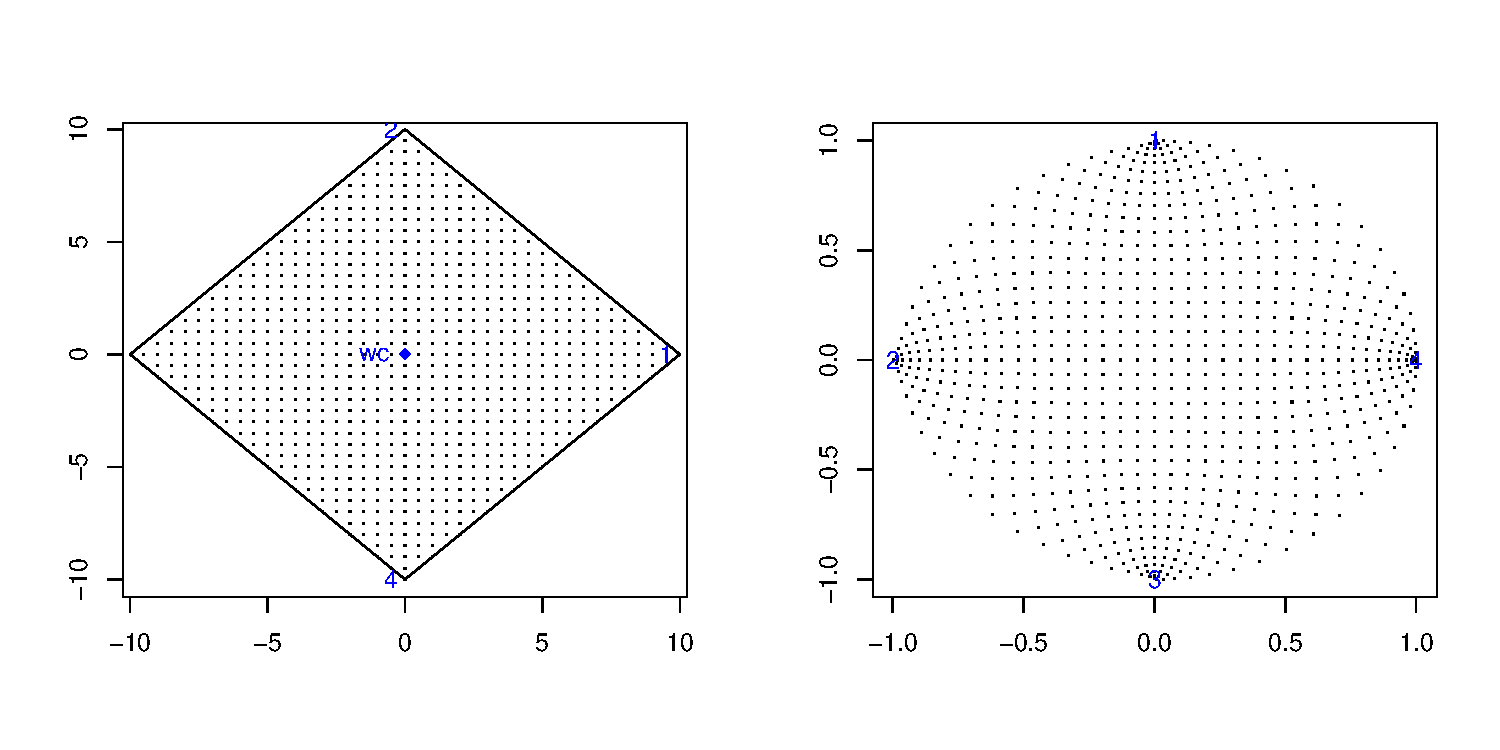
\includegraphics[scale=0.5]{sc/figs/squaredomain.pdf}
\caption{The left panel shows a regular grid of points over the square region. The right panel shows the mapping of these points under the \sch transformation to the unit disk.}
\label{squaredomain}
\end{figure}

% Irregular mapping diagram
\begin{figure} [tbp]
\centering
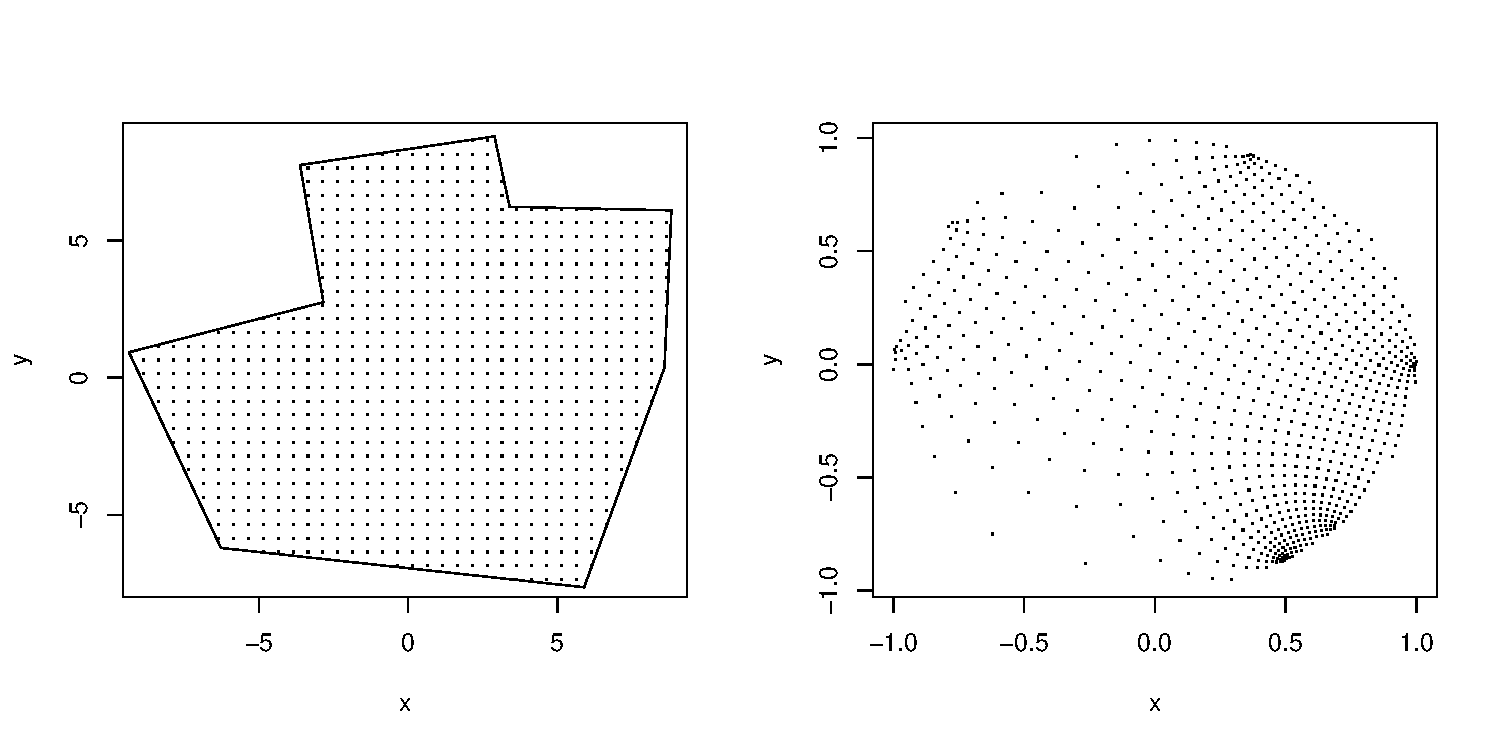
\includegraphics[scale=0.5]{sc/figs/irregulardomain.pdf}
\caption{The left panel shows a regular grid of points over region bound by a irregular nonagon. The right panel shows the mapping of these points under the \sch tranformation to the unit disk.}
\label{irregdomain}
\end{figure}

\subsection{Crowding}

\subsubsection{The crowding problem}
When the polygon is elongated or has many vertices, the mapped vertices may be positioned too closely in the transformed domain. This effect is referred to as \emph{crowding} and can be observed in \fig{crowdeddisk}. In elongated regions prevertices can be located exponentially close such that they are indistinguishable in finite precision arithmetic (\cite{howell90}.)

% Crowded mapping diagram
\begin{figure} [tbp]
\centering
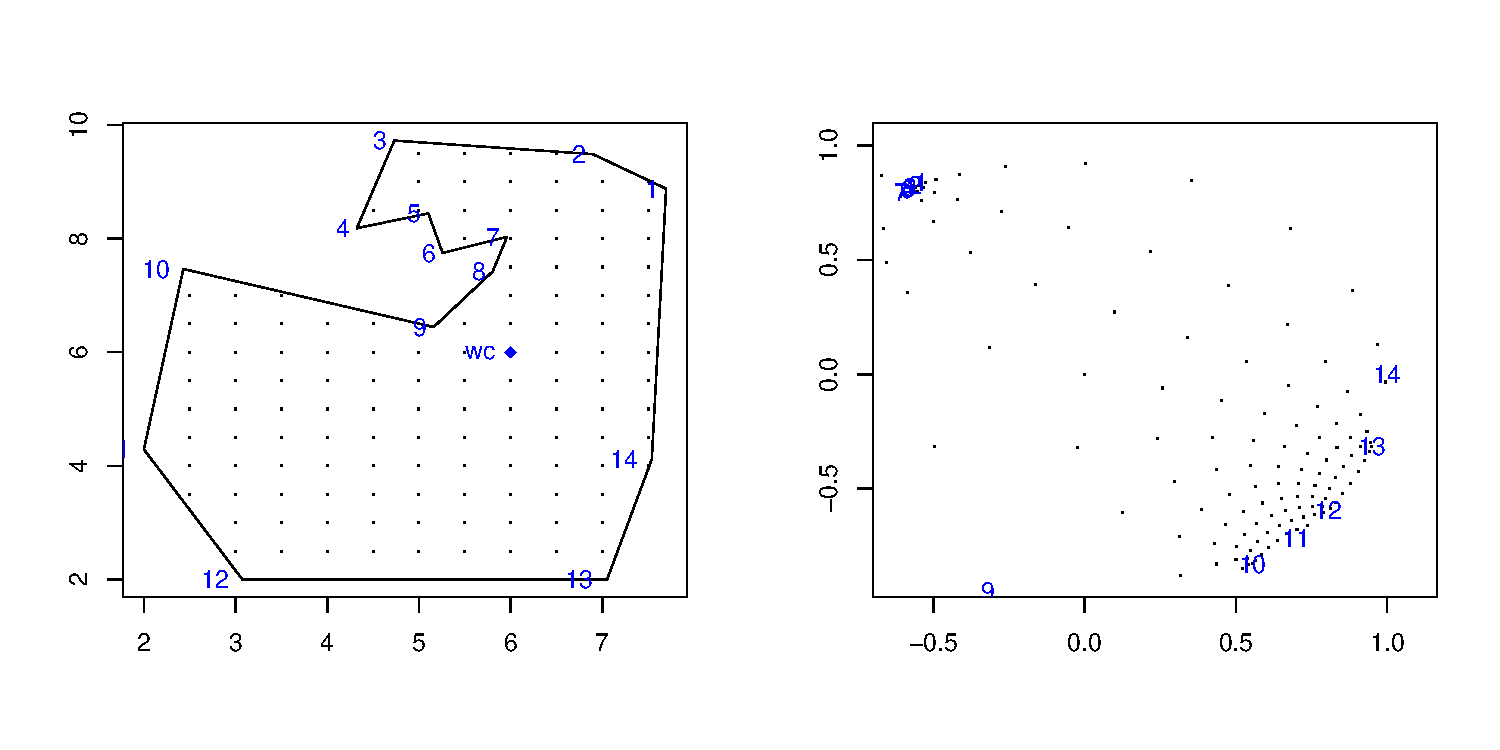
\includegraphics[scale=0.5]{sc/figs/crowdeddisk.pdf}
\caption{An example of crowding. Note that prevertices 1 through 8 are mapped to a single point in the right panel and their relative proximity in the left panel.}
\label{crowdeddisk}
\end{figure}

\subsubsection{Fixing crowding}

If the crowding is caused by $\Gamma$ being elongated then a  primitive fix is to map to an elongated domain such as the rectangle or plane. This approach is suggested in \cite{howell90} however, as they point out, this does not eliminate all crowding and problems can still occur when there are strongly acute peninsulae in the polygon. Mapping to an elongated domain also does not fix problems which occur when mapping from T- or H-shaped domains (so-called ``multiply elongated'' domains.)

In order to combat this problem more effectively, \cite{vavasis96} propose the CRDT (cross-ratios of the Delaunay triangulation) algorithm. Each set of prevertices has $n-3$ degrees of freedom hence, there is a three parameter family of possible vertex arrangements that all map to the same polygon. The most stable of these \emph{embeddings} should be used. The M\"{o}bius transformation relates the embeddings to one another.

We can extend this idea further by noting that the polygon is identical if additional vertices are added between the current ones, provided that the internal angle associated with the new vertex is $\pi$. These extra vertices also do not change the \sch formula since in \eqn{unitscmap} $\alpha_k=1$ for an angle of $\pi$. Adding these extra vertices allows us to control the aspect ratio of the map.

In the solution to the \sch parameter problem given in \ref{sc-parprob}, conditions on the side lengths and orientations of the polygon are enforced. Instead, the CRDT algorithm imposes conditions about quadrilateral sections of the polygon and the diagonals of the polygon. We can do this by first performing a Delaunay triangulation of the domain and then merging pairs of triangles into a quadrilateral. A measure is then defined (the \emph{cross-ratio}) which specifies a set of non-linear equations to be solved. These equations enforce the constraint that the cross-ratio in mapped polygon comes out correctly. 

Putting all of these ideas together gives the CRDT algorithm. We first add edges to the polygon with internal angle $\pi$ to remove enlongated parts of the domain and then triangulate the domain. Once the domain is triangulated we calculate the cross-ratio:
\begin{equation}
\rho(a,b,c,d) = \frac{(d-a)(b-c)}{(c-d)(a-b)},
\end{equation}
for each quadrilateral in the polygon. Then, analogously to \eqn{optimizeme} we set up a series of equations, specifying that the cross-ratios remain the same in the polygon and the transform of the rectangle back to the polygon. We then wish to solve for the values of $\rho$ for the original domain in the same manner as we solved for side lengths in the original problem. 

We can see in \fig{uncrowdeddisk} that when the CRDT method is used with a rectangular domain that the crowding has been alleviated. The point density, as well as vertex density seems to be more uniform than in \fig{crowdeddisk}.

% Uncrowded mapping diagram
\begin{figure} [tbp]
\centering
\includegraphics[scale=0.5]{sc/figs/irregular-fixed-crdt.pdf}
\caption{The mapping of the irregular domain featured in \fig{crowdeddisk} using the CRDT method mapping to a rectangle. The crowding is now much less severe.}
\label{uncrowdeddisk}
\end{figure}

The downside of using CRDT is that it may add too many vertices to maintain the aspect ratio (\cite{driscoll05},) so the algorithm tends to take longer than the one specified in Section (\ref{algorithmsketch}) since it is $O(n^3)$ JUSTIFY AND ELABORATE ON THIS!. This is, of course, offset against the fact that the problem becomes tractable.






\section{Simulation experiments}

In order to test the efficacy of the \sch transform for the purposes of smoothing over complex regions, a series of simulation experiments were performed.

\bi
	\item Software
	\item which domains
	\item results
\ei


There are several pieces of software available to perform the \sch mapping. The Fortran library \texttt{SCPACK} is the oldest available package\footnote{\texttt{SCPACK} can be downloaded from Netlib.} and was used initially. However, it only offers the mapping to the unit disk and does not include the CRDT method for performing the mapping (see \cite{miller08}, section (4.2).) For this reason the SC toolbox (\cite{driscoll}, \emph{pp. 115-119}) for Matlab is used to perform the mapping. 

The \textsf{R} library \texttt{mgcv} provides subroutines for fitting generalized additive models and, in particular, P-splines.

Although packages are available to enable \textsf{R} to talk to Matlab and vice-verse, for the purposes of this exploratory work CSV files were written by each program and read in by the other.

\subsection{Ramsay horseshoe}

The first and most obvious candidate for simulation is the modified Ramsay horseshoe (described in depth in chapter THE CHAPTER, section THE SECTION.)

In order to map the horseshoe, we first draw a rough bounding box around the shape. Rather than trying to approximate the curved edges with many straight lines, we use the bounding box as the $W$ domain remapped via the \texttt{evalinv()} function from the \emph{SC Toolbox}. This is shown in \fig{hswithboundingbox}.

We then transform our bounding box into the rectangle. This is done using the \texttt{rectmap()} or \texttt{crrectmap} (its CRDT equivalent) function from the \emph{SC Toolbox} in Matlab. This function solves the \sch parameter problem as detailed in \ref{schparprob}. A sample of 1000 points was then taken from the horseshoe and noise added to the data. First the $x$,$y$ coordinates of the sampled points were expressed as complex numbers of the form $w=x+iy$. The mapping was then performed. This created a new set of coordinates $w^*=x^*+iy^*$. Smoothing was then performed over the responses in the $W^*$ domain using the \texttt{gam()} function in \texttt{mgcv}. 

\begin{figure}
\centering
% trim order l b r t
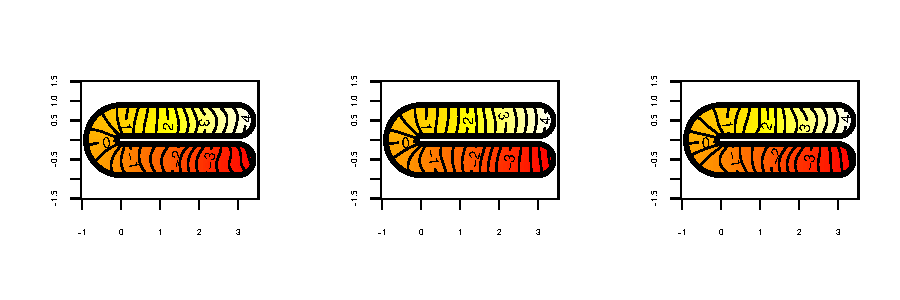
\includegraphics[trim=0.5in 0.5in 0in 0in]{sc/figs/compsmooth.pdf} \\
\caption{Comparison of smooths given using P-splines on the transformed domain (left), thin plate splines on the transformed domain (centre) and soap film smoother (right.)}
\label{compsmooth}
% generated by /phd-smoothing/sc-writeup/figs/pspline.soap.comp.hs.R
\end{figure}

CHANGE THIS FIGURE!!!! WANT TO HAVE A 2 by 2 plot!!!!
\Fig{compsmooth} shows the true function and typical realisations of: the fit given using a \tprs without transformation, the fit given by a \tprs with transformation and the fit given by the soap film smoother. From looking at these heat maps one can see that the \sch transform is clearly making the \tprs perform better. However, visual inspection alone is clearly not enough basis for accepting the method, therefore we now look at the mean squared error of the models.

\begin{table}[ht]
\begin{tabular}{c c}\\
Sample size & Noise level$^{1}$ \\
\hline
\hline
1000 & 0.3 \\
500 & 0.3 \\
250 & 0.3 \\
100 & 0.3 \\
1000 & 0.5 \\
1000 & 1 \\
1000 & 2 \\
\end{tabular}
\caption{Setup for the simulations. $^{1}$Noise level is noise added to the test function from a standard Normal multiplied by the value in this column.}
\label{scramsimtable}
\end{table}

\Tabref{scramsimtable} shows the settings for noise level and sample size of the simulations. Mean squared error between the true function and the fitted model was used to evaluate the model's performance. In the following tables we provide the mean squared error over a prediction grid of 1000 points averaged over 1000 generated data sets.

\Tabref{scramsayres} shows the results from the simulations for the standard horseshoe. A cursory glance show that that results were better than those for the soap film smoother for larger sample sizes and standard errors were comparable. Once we get to 100 samples the method performance degrades over all methods. Once noise is introduced into the data we can see that the soap film and transformation method do as well as each other, MSEs are approximately the same and the standard errors are of the same order.

SAY SOMETHING ABOUT THE BOXPLOTS. THEY NEED TO BE REGENERATED!!!!

\begin{figure}
\centering
% trim order l b r t
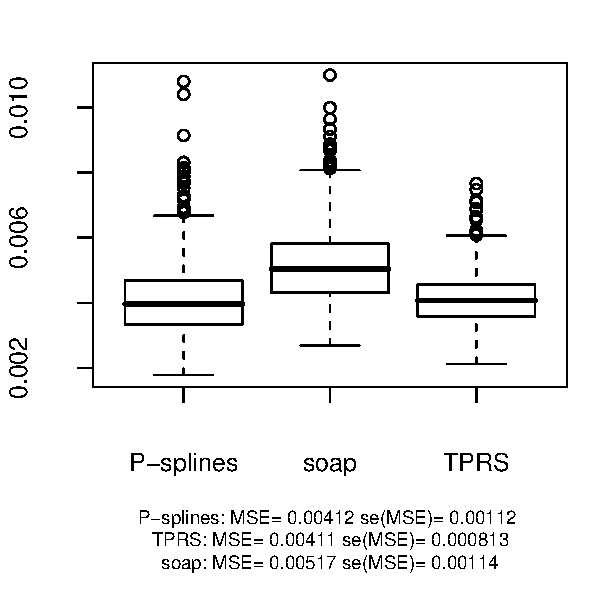
\includegraphics{sc/figs/mses-boxplot.pdf} \\
\caption{Boxplots of mean MSE from 1000 points on a prediction grid from 1000 simulations.}
\label{scram1000boxplots}
% generated by ramsaysim/makeboxplots.R
\end{figure}

\begin{table}[ht]
\begin{tabular}{c c c c c}\\
Sample size & Noise level & P-spline MSE (\emph{sd}) & Thin plate MSE (\emph{sd}) & Soap MSE (\emph{sd}) \\
\hline
\hline
1000 & 0.3 & 0.00412 (0.00112) & 0.00811 (0.00243) & 0.00517 (0.00114) \\ 
500 & 0.3 & 0.00505 (0.00144) & 0.00478 (0.000955) & 0.00628 (0.00146) \\ 
250 & 0.3 & 0.00875 (0.00392) & 0.00684 (0.00183) & 0.0107 (0.00305) \\ 
100 & 0.3 & 0.0225 (0.035) & 0.0118 (0.00461) & 0.0219 (0.0117) \\ 
1000 & 0.5 & 0.0105 (0.00353) & 0.00811 (0.00243) & 0.0127 (0.0034) \\ 
1000 & 1 & 0.0242 (0.0108) & 0.0161 (0.0069) & 0.0275 (0.00958) \\ 
1000 & 2 & 0.066 (0.0481) & 0.0388 (0.0229) & 0.0686 (0.0333) \\ 
\end{tabular}
\label{scramsayres}
\caption{Mean squared error along with its standard deviation for the transformed Ramsay horseshoe (for P-spline and thin plate cases) versus those for the soap film smoother.}
% generated by /phd-smoothing/sc-writeup/tablecode/ramsay.sim.results.table.R
\end{table}






















Looking at the predicted values for the model in the $W^*$ domain we get an indication as to why the fit is so good. \Fig{hsvisgam} shows the fitted surface and there we can see that there is a strong linear trend along the major axis of the horseshoe, making this a rather trivial smoothing problem. So, it looks like we are addressing the problem in a more natural domain. In the next section we investigate this further.

\begin{figure}
\centering
% trim order l b r t
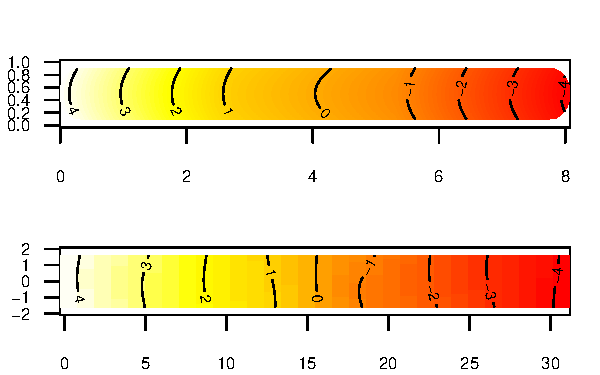
\includegraphics[trim=0in 0.5in 0in 0in]{figs/hsvisgam.pdf} \\
\caption{Heatmap produced by \texttt{vis.gam} for the smooth over the horseshoe in the transformed domain using P-splines (left) and thin plate splines (left).}
\label{hsvisgam}
% generated by /phd-smoothing/sc-writeup/figs/hsvisgam.R
\end{figure}

\subsection{Problems}

As mentioned above, when the domain has been morphed it is not clear what the definition of smoothness is, \emph{ie.} determining the nullspace of the penalty term. In this respect we would like to find out about the distortion to space caused by the transform. In order to do this we take a straight line in the domain and see what it maps to in the $W^*$ domain. We can also look at the response along that line according to the transformed and untransformed coordinate systems and see how this compares to looking at the response in the horseshoe's natural coordinate system.

\Fig{horseshoecentreline} shows the line that was evaluated along the centre of the horseshoe and its equivalent line in the transformed domain. We can see from this that a line that is straight in the domain appears to be bent in the transform. The curvature does not appear to be particularly extreme in this case, however, one can imagine that this could get significantly worse for regions with more complicated boundaries.

We may also look at the response along the centre line. \Fig{centrelinelineplot} shows the evaluations of the horseshoe function over the line plotted against three coordinate systems. The first plot shows the function evaluations on the $W$ domain as a response to change in $y$. The second on the $W^*$ domain, as a response to $y^*$, the transformed coordinate system. The final plot is in the horseshoe's ``natural'' domain, \emph{ie.} the value the horseshoe takes as a function of distance along the major axis of the shape.

\begin{figure}
\centering
% trim order l b r t
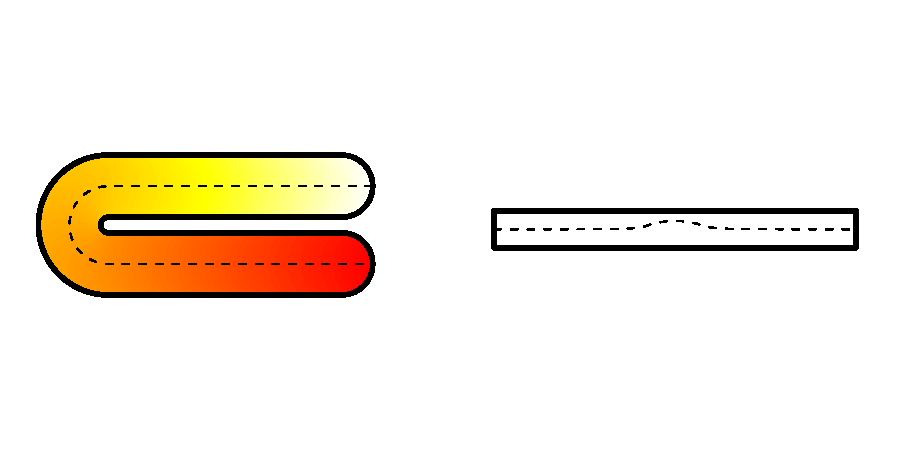
\includegraphics[trim=0.5in 1in 0in 1in]{figs/horseshoecentreline.pdf} \\
\caption{The dashed line here gives the centre line that we will map to investigate the smoothness under the \sch transform. The left figure gives the untransformed domain and the right the one that has undergone the transformation.}
\label{horseshoecentreline}
% generated by /phd-smoothing/ramseysim/nullspace.test.R 
\end{figure}


\begin{figure}
\centering
% trim order l b r t
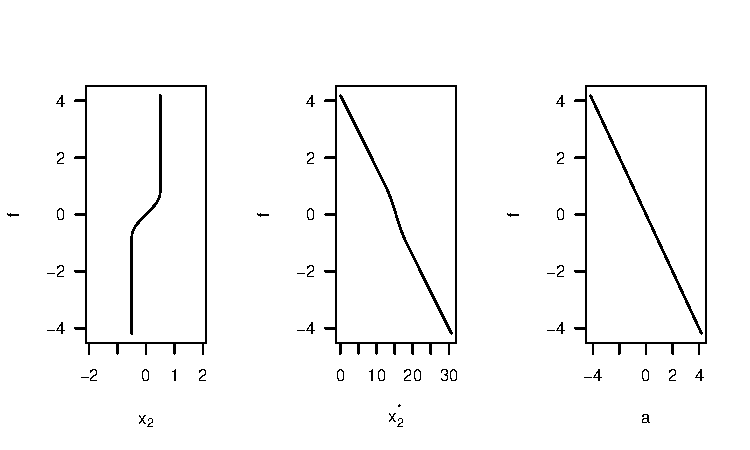
\includegraphics[trim=0in 0in 0in 0in]{figs/centrelinelineplots.pdf} \\
\caption{Plots of the horseshoe function against the $y$ axis for (left) the untransformed horseshoe, (middle) the shape under the \sch transform and, (right) the function evaluation against the major axis.}
\label{centrelinelineplot}
% generated by /phd-smoothing/ramseysim/nullspace.test.R 
\end{figure}

From these plots one can see that the \sch transform approximates the natural domain of the horseshoe quite well, with only two minor kinks in the line. Looking at where the kink occurs, it corresponds exactly with the kink in \fig{horseshoecentreline}. This makes sense, since we would expect a change in gradient if direction we are traveling has moved into two dimensions from one.

We now return to our original question of the nullspace of the penalty. The original Ramsay test function is given by a simple gradient in the direction of the major axis of the horseshoe. This function would not be penalized, as it is just a straight line (and hence its second derivative is zero.) We can see from \fig{centrelinelineplot} that in the natural domain of the horseshoe the line is straight and that this is almost the case in the transformed domain. Hence we can conclude that in this case the nullspace is almost the same as that in the natural domain.














 the second with a gradient across the short axis of the horseshoe. This second test function can be seen in \fig{altramsayhorseshoe}. Table (\ref{simtable}) shows the setup of these experiments, which were run on both test functions.

\begin{figure}
\centering
% trim order l b r t
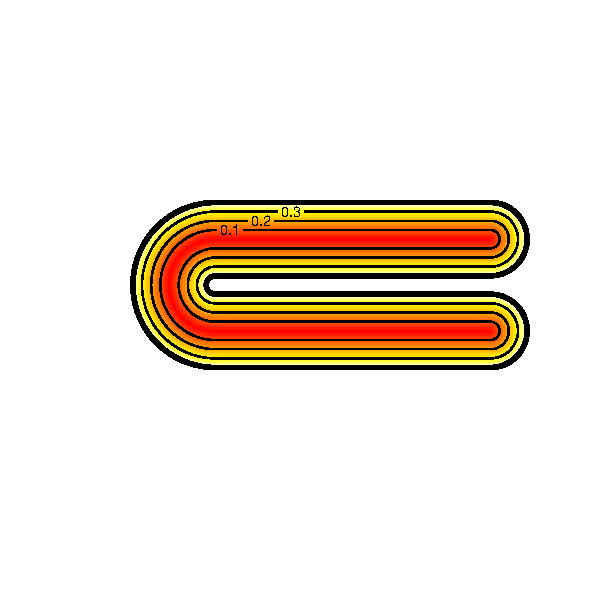
\includegraphics[trim=0.5in 1in 0in 0.5in]{figs/altramsayhorseshoe.pdf} \\
\caption{Heatmap of the alternate version of the Ramsay horseshoe.}
\label{altramsayhorseshoe}
\end{figure}




For the alternative horseshoe we begin to see the soap film creep ahead of the transformation method (see table (3).) Although the MSEs are of approximately the same order (as are the standard errors), the soap film is gaining ground. To examine what is going on here we can look at the plots of the predicted values as heat maps. These can be seen in \fig{altramsaycomp} and show that the \sch mapping seems to capture the overall structure of the shape better than the soap film smoother, which seems to capture patches of the shape but not the overall structure. It also appears that the \sch method does not respect the ends of the horseshoe and continues the gradient running along the minor axis over this part as well.This feature seems to be the cause of the performance decrease.

\begin{table}[ht]
\begin{tabular}{c c c c c}\\
Sample size & Noise level & P-spline MSE (\emph{sd}) & Thin plate MSE (\emph{sd}) & Soap MSE (\emph{sd}) \\
\hline
\hline
1000 & 0.3 & 0.00415 (0.00117) & 0.0158 (0.00247) & 0.00378 (0.00108) \\ 
500 & 0.3 & 0.00469 (0.00147) & 0.00793 (0.00186) & 0.00458 (0.00145) \\ 
250 & 0.3 & 0.00716 (0.00431) & 0.0142 (0.00249) & 0.00771 (0.00301) \\ 
100 & 0.3 & 0.039 (0.22) & 0.0201 (0.00589) & 0.0298 (0.42) \\ 
1000 & 0.5 & 0.00839 (0.00403) & 0.0158 (0.00247) & 0.00966 (0.00371) \\ 
1000 & 1 & 0.0194 (0.0122) & 0.0226 (0.0085) & 0.019 (0.00981) \\ 
1000 & 2 & 0.0605 (0.0468) & 0.0436 (0.0276) & 0.041 (0.0434) \\ 
\end{tabular}
\label{altramsayresultstable}
\caption{Mean squared error along with its standard deviation for the transformed alternate Ramsay horseshoe (for P-spline and thin plate cases) versus those for the soap film smoother.}
% generated by /phd-smoothing/sc-writeup/tablecode/alt.ramsay.sim.results.table.R
\end{table}

\begin{figure}
\centering
% trim order l b r t
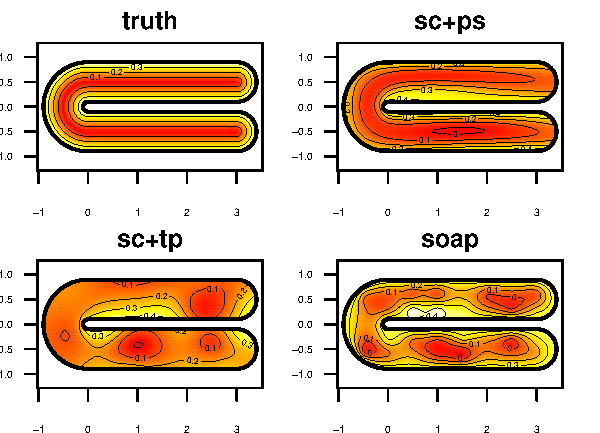
\includegraphics[width=5in, trim=0in 0in 0in 0in]{figs/altramsaycomp.pdf}\\
\caption{Single realizations of the fit to the alternate Ramsay horseshoe for each method. Clockwise from top left: the original figure, the function estimated by the \sch transform with P-splines, function estimated by the \sch transform with thin plate splines and finally the soap film estimate.}
\label{altramsaycomp}
% generated by /phd-smoothing/sc-writeup/figs/altramsaycompare.R 
\end{figure}

\Fig{altcentrelinelineplot} shows analogous plots to \fig{centrelinelineplot} and backs up this hypothesis. The second panel shows the mapping of the $y$ component of the centreline against the response and the third panel shows the same in the horseshoe's own domain. It appears that the two plots are indistinguishable.

\begin{figure}
\centering
% trim order l b r t
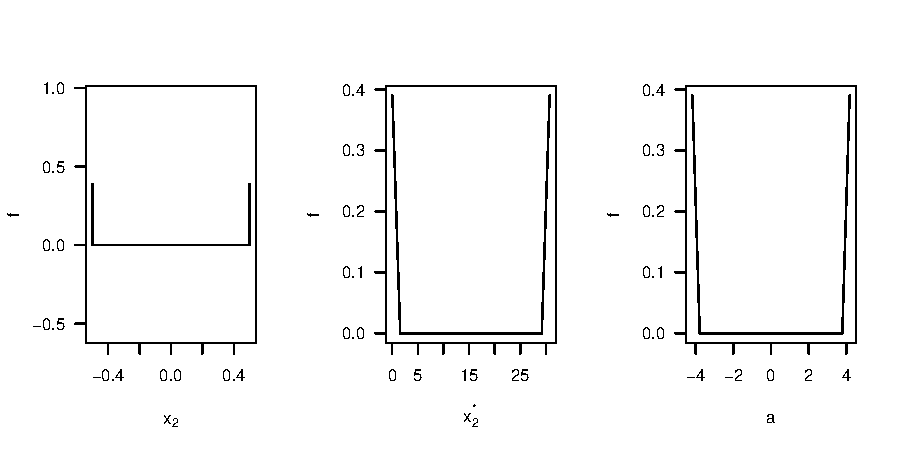
\includegraphics[trim=0in 0in 0in 0in]{figs/altcentrelinelineplots.pdf} \\
\caption{Plots of the alternate horseshoe function against the $y$ axis for (left) the untransformed horseshoe, (middle) the shape under the \sch transform and, (right) the function evaluation against the major axis.}
\label{altcentrelinelineplot}
% generated by /phd-smoothing/altramsaysim/nullspace.test.R 
\end{figure}



















\section{Conclusions \& Analysis}


\begin{figure}
\centering
% trim order l b r t
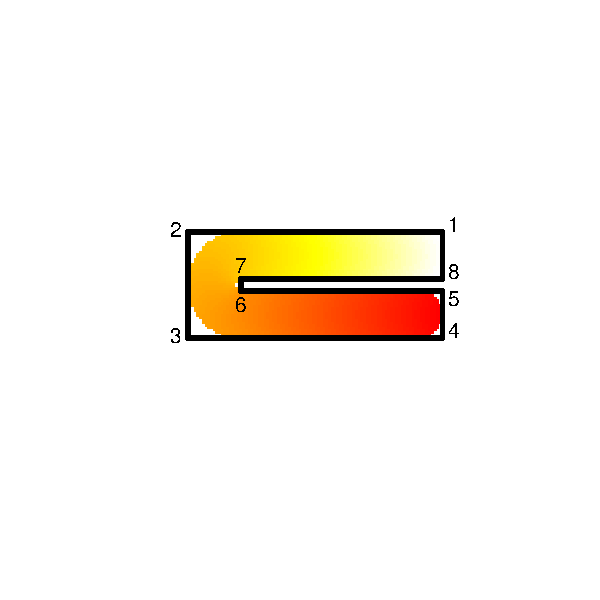
\includegraphics[trim=0.5in 1in 0in 1in]{sc/figs/hswithboundingbox.pdf} \\
\caption{The horseshoe with it's bounding box. The vertices marked 1, 4, 5 and 8 are mapped to the corners of the rectangle.}
\label{hswithboundingbox}
% generated by /phd-smoothing/sc-writeup/figs/hswithboundingbox.R
\end{figure}






Why this doesn't work but why it wasn't a waste of time.
